\documentclass[12pt]{article}

\usepackage{graphicx}%
\usepackage{multirow}%
\usepackage{amsmath,amssymb,amsfonts,bbm,bm}%
\usepackage{amsthm}%
\usepackage{mathrsfs}%
\usepackage[dvipsnames,svgnames,x11names]{xcolor}%
\usepackage{booktabs}%
\usepackage{algorithm,algorithmicx,algpseudocode}%
\makeatletter\renewcommand{\theHALG@line}{\thealgorithm.\arabic{ALG@line}}\makeatother
\usepackage{natbib}%
\bibliographystyle{agsm}
\usepackage{hyperref,xurl}
\hypersetup{
  colorlinks=true,
  linkcolor={blue},
  filecolor={Maroon},
  citecolor={Blue},
  urlcolor={Blue}
}
\usepackage[capitalize,nameinlink]{cleveref}
\usepackage{subfig}
\usepackage[margin=2cm]{geometry}
\usepackage[no-weekday]{eukdate}
\usepackage{caption}
\captionsetup{labelfont=bf,textfont=it}

\raggedbottom\sloppy
\allowdisplaybreaks
\clubpenalty=10000
\widowpenalty=10000

\newcommand{\R}{\mathbb{R}}
\renewcommand{\P}{\mathbb{P}}
\newcommand{\E}{\mathbb{E}}
\newcommand{\diag}{\text{diag}}

\theoremstyle{plain}%
\newtheorem{theorem}{Theorem}
\newtheorem{lemma}{Lemma}
\newtheorem{proposition}{Proposition}
\newtheorem{remark}{Remark}
\newtheorem{counterexample}{Counterexample}
\newtheorem{corollary}{Corollary}
\theoremstyle{definition}
\newtheorem{defn}{Definition}

\crefname{defn}{Definition}{Definitions}
\Crefname{defn}{Definition}{Definitions}
\crefname{counterexample}{Counterexample}{Counterexamples}
\Crefname{counterexample}{Counterexample}{Counterexamples}
\crefname{proposition}{Proposition}{Propositions}
\Crefname{proposition}{Proposition}{Propositions}

\renewcommand{\sectionautorefname}{Section}
\renewcommand{\subsectionautorefname}{Section}
\renewcommand{\subsubsectionautorefname}{Section}
\newcommand{\corollaryautorefname}{Corollary}
\newcommand{\lemmaautorefname}{Lemma}

\graphicspath{{Figures/}}

\def\spacingset#1{\renewcommand{\baselinestretch}%
{#1}\small\normalsize}

\begin{document}

\spacingset{1}

%%%%%%%%%%%%%%%%%%%%%%%%%%%%%%%%%%%%%%%%%%%%%%%%%%%%%%%%%%%%%%%%%%%%%%%%%%%%%%

\title{\bf Lookout 2: Anomaly Detection via Leave-One-Out Kernel Density Estimation}
\author{
  Rob J Hyndman\\
  Department of Econometrics and Business Statistics, Monash University,\\
  Clayton VIC 3800, Australia\\
  Email: rob.hyndman@monash.edu\\
  and\\
  Sevvandi Kandanaarachchi\thanks{Corresponding author.}\\
  CSIRO Data61, Clayton VIC 3168, Australia\\
  Email: sevvandi.kandanaarachchi@csiro.au\\
  and\\
  Katharine Turner\\
  Mathematical Sciences Institute, Australian National University,\\
  Canberra ACT 2601, Australia\\
  Email: katharine.turner@anu.edu.au
}
\maketitle

\bigskip
\begin{abstract}
  The lookout algorithm identifies anomalies in multivariate data by fitting a generalized Pareto distribution to the largest surprisals (negative log densities) of a leave-one-out kernel density estimate. Its bandwidth is chosen by persistent homology, using death diameters equivalent to the edge lengths of the Euclidean minimum spanning tree. We use the tree to analyse the algorithm and propose three changes. First, a robust covariance standardization replaces min-max scaling. Second, the bandwidth is set using an upper quantile of the edge lengths in place of the edge length below the largest gap between consecutive lengths. Third, the generalized Pareto shape parameter is constrained to be non-positive. Using limit theory for random geometric graphs, we show that the scaled quantile converges in probability to a constant for any density, so the bandwidth has the order of the spacing between neighbouring observations in the sparse part of the sample. The longest edges, which the original bandwidth typically uses, grow without bound under heavy tails. Neither bandwidth gives a consistent density estimate in general; we argue that the modified one behaves appropriately for anomaly detection. In simulations and two applications, the modified algorithm usually improves on the original and compares well with other methods.
\end{abstract}

\noindent%
\textit{Keywords:}
bandwidth selection,
extreme value theory,
generalized Pareto distribution,
minimum spanning tree,
outlier detection.

\newpage
\spacingset{1.8} % DON'T change the spacing!

% -----------------------------------------------------------
\section{Introduction} \label{sec:intro}
% ------------------------------------------------------------

Two contributions: 1. theoretical properties of lookout algorithm \citep{lookoutori}; and 2. modified lookout algorithm with better properties and performance.

\subsection{The lookout algorithm for anomaly detection (SK)}
The \textit{lookout}  algorithm has 3 inputs: the dataset $\bm{X}$ containing $N$ data points in $\mathbb{R}^p$, a parameter $\alpha \in (0,1)$ signifying the cut-off for the Generalized Pareto Distribution (GPD) and a binary variable \textit{unitize} which tells the algorithm whether to normalize the data or to keep it as it is. We briefly outline the steps below.

% Given a set of $N$ points in $\mathbb{R}^p$ denoted by $\bm{X}$ and a parameter $\alpha \in (0,1)$ signifying the upper bound for the proportion of anomalies, \textit{lookout} finds anomalies as follows:
\begin{enumerate}
    \item If \textit{unitize} = TRUE, then normalize $\bm{X}$ using min-max scaling so that normalized data lies in the unit cube in $\mathbb{R}^p$.
    \item Construct the persistence homology barcode of the data cloud for dimension zero using the Vietoris-Rips diameter. From the barcode we obtain the death diameters $\{d_i\}_{i = 1}^N$ for connected components. We compute successive differences $\Delta d_i = d_{i+1} - d_i$ for $i \in \{1, \ldots , N\}$ and choose the diameter $d_i$ corresponding to the maximum $\Delta d_i$. That is, $i_{*} = \arg max \{ \Delta d_i \}_{i=1}^N$ and  $d_{*} = d_{i_*}$.
    \item Using $\bm{H} = (d_*)^{2/p} \bm{I}$, we compute kernel density estimates $\hat{f}(\bm{x}; \bm{H}) = \frac{1}{N} \sum_{i = 1}^N K_{\bm{H}}(\bm{x} - \bm{x}_i) $ using the multivariate scaled Epanechnikov kernel  $K(\bm{x}) = \frac{p+2}{ c_p}(1 - \lVert x \rVert^2/5)_+$ where  $c_p$ is the volume of the unit sphere in $\mathbb{R}^p$ and $u_+ = \max(0, u)$. Using $\hat{f}(\bm{x}; \bm{H})$ we compute the leave-one-out kernel density estimates $\hat{f}_{-j}(\bm{x}_j; \bm{H}) = \frac{1}{N-1} \left( N \hat{f}(\bm{x}_j; \bm{H}) - \bm{H}^{-1/2} K(\bm{0}) \right) $.
    \item Let $y_i$ and $y_{-i}$ be the kde and leave-one-out kde of $\bm{x}_i$ respectively. 
    \item Using the Peak Over Threshold (POT) approach, fit a Generalized Pareto Distribution (GPD) to $\left\{ - \log y_i \right\}_{i = 1}^N$ and estimate the location, scale and shape parameters of the GPD $\mu$, $\sigma$ and $\xi$. 
    \item Using the estimated GPD  parameters $\hat{\mu}$, $\hat{\sigma}$ and $\hat{\xi}$ find the probability of the leave-one-out kde values $\left\{ - \log y_{-i}.  \right\}_{i = 1}^N$. This is the probability of observing the datapoints given the estimated GPD parameters $P\left(- \log y_{-i} | \hat{\mu}, \hat{\sigma}, \hat{\xi} \right)$. 
    \item If $P\left(- \log y_{-i} | \hat{\mu}, \hat{\sigma}, \hat{\xi} \right) < \alpha$ declare $\bm{x}_i$ as anomalous.     
\end{enumerate}
The output of \textit{lookout} is the list of anomalies, their GPD probabilities, the anomaly scores computed as $1 - P\left(- \log y_{-i} | \hat{\mu}, \hat{\sigma}, \hat{\xi} \right)$, the bandwidth computed using $d_*$, the kde values $\{y_i\}_{i=1}^N$, the leave-one-out kde values $\{y_{-i}\}_{i=1}^N$ and the estimated GPD parameters. More details of this approach are given in \cite{lookoutori}. 
% 

\subsection{Consistency of kde when bandwidths use Rips death diameters (RH)}

Suppose we have a sample of $n$ points in $\mathbb{R}^p$, and we want to estimate the density of the underlying distribution $f$ using a multivariate kernel density estimator with the bandwidth matrix $\bm{H}$.

Let $d_1,\dots,d_N$ denote the (ordered) Rips death diameters computed from the sample $\bm{y}_1,\dots,\bm{y}_N$, and let
$$
	d_* = d_{i_*}\qquad\text{where}\quad i_* = \text{arg max}\{d_{i+1} - d_i\}_{i=1}^{N-1}
$$
That is, $d_*$ is the Rips diameter corresponding to the lower point of the largest gap in the Rips diameters. Then the bandwidth matrix proposed by \cite{lookoutori} is given by
\begin{equation}\label{eq:bandwidth}
	\bm{H} = d_*^{2/p}\bm{I},
\end{equation}
where $p$ is the dimension of the data. \citet{lookoutori} demonstrated the results of their algorithm on a variety of simulated and real datasets, but did not provide a theoretical justification for their choice of bandwidth. In this paper, we revisit the issue and establish some conditions under which this choice of bandwidth provides a consistent estimator of the density. As a result, we propose a modification of the bandwidth selection method, leading to a lookout algorithm that works under a much broader range of conditions.

To obtain a consistent estimator, we need $\bm{H}$ to be positive definite and symmetric, and to satisfy the following conditions \citep[][p31--37]{chacon2018multivariate}:
\begin{itemize}
	\item All elements of $\bm{H}$ approach zero as $n\rightarrow\infty$; and
	\item $n^{-1}|\bm{H}|^{-1/2} \rightarrow 0$ as $n\rightarrow\infty$.
\end{itemize}
Thus, for the approach of \cite{lookoutori} to work, we need to show that
\begin{equation}\label{eq:conditions}
	d_*^{2/p}\rightarrow 0 \quad\text{and}\quad (d_*n)^{-1}\rightarrow0\quad{as}\quad
	n\rightarrow\infty
\end{equation}

\subsection{Crackle (KT)}

Describe crackle idea and why it matters here

\subsection{The modified lookout algorithm (RH)}

As a result of these theoretical considerations, we propose several modifications to the lookout algorithm.
\begin{enumerate}
	\item Rather than use the lower point of the largest gap in Rips death diameters, we propose to use an upper quantile of the Rips death diameters. This avoids the problem where anomalies affect the largest Rips diameters.
	\item We propose to use a Yeo-Johnson transformation on the margins of the distribution, to avoid the problem of distributions with heavy tails.
	\item Finally, we scale and rotate the transformed data to ensure that the data have zero pairwise correlations. This better aligns the bandwidth matrix to the data.
\end{enumerate}
Note that we do not need to estimate the density of the underlying distribution directly. Instead, we can estimate the density of a transformation of the data, and identify anomalies in the transformed space. Hence, there is no need to undo the scaling, rotation or Yeo-Johnson transformation.


% -----------------------------------------------------------
\section{Bandwidth selection from the minimum spanning tree} \label{sec:mst}
% ------------------------------------------------------------

\subsection{The bandwidth rule}

Let $T$ denote the Euclidean minimum spanning tree of $\{\bm{y}_1,\dots,\bm{y}_n\}\subset\R^m$: the connected graph on the $n$ observations whose total edge length is smallest. Provided the pairwise distances are distinct, which holds almost surely when the observations are drawn from a continuous density, $T$ is unique and has $n-1$ edges. When placed in increasing order, the edge lengths are denoted by $e_{(1)} \le \cdots \le e_{(n-1)}$.

\begin{defn}[Minimum spanning tree bandwidth]\label{def:mstbw}
  For $\gamma\in(0,1)$, the \emph{minimum spanning tree bandwidth} is the $\gamma$ quantile of the edge lengths of $T$,
  \begin{equation}\label{eq:mstbw}
    h_n = e_{(\lceil \gamma(n-1)\rceil)}.
  \end{equation}
\end{defn}
We take $\gamma = 0.98$ throughout unless stated otherwise. (In computation, we use the median-unbiased quantile estimator of \citet{HF96} rather than the order statistic itself, but the distinction is immaterial asymptotically.) The kernel density estimate \eqref{eq:mkde} is then computed with the bandwidth matrix
\begin{equation}\label{eq:Hmst}
  \bm{H} = ah_n^2\bm{I}_m,
\end{equation}
where $a=m+4$ for the Epanechnikov kernel.

The single linkage reading of \eqref{eq:mstbw} assists interpretability. Cutting the single linkage dendrogram at height $h_n$ splits the $n$ observations into about $(1-\gamma)n$ connected components. With $\gamma=0.98$, the bandwidth is the scale at which single linkage has gathered all but about 2\% of the observations into components. It is a measure of how far apart neighbouring observations are once the few most isolated ones are set aside.

To compute $h_n$, we use the dual-tree Bor\r{u}vka algorithm of \citet{March2010}, as implemented in \texttt{mlpack} \citep{mlpackR}, which builds the exact Euclidean minimum spanning tree in $O(n\log n)$ time under the same assumptions that make dual-tree nearest-neighbour search efficient, and degrades gracefully in higher dimensions.

% TODO (step 4): three-panel figure --- 2-d point cloud with its MST, the single
% linkage dendrogram with the gamma cut marked, and the resulting KDE contours
% with the detected anomalies.

% TODO (step 4): timing table or figure over n and m, and the measured cost
% against a Rips filtration. Needs new R scripts and targets.

\subsection{Other uses of MST in anomaly detection}\label{sec:related}

Minimum spanning trees have a long history in multivariate statistics, and we are not the first to use them in an anomaly detection context.
\citet{Rohlf1975} gave the classical minimum spanning tree test for multivariate outliers. When $m=1$, the edges of the minimum spanning tree are the gaps between consecutive order statistics, so the edge lengths of the tree are the natural multivariate generalization of the univariate gap test; Rohlf tests the largest squared edge length, divided by the mean squared edge length, against a gamma null distribution. However, \citet{caroni1995rohlf} argue that this is not a useful formal test.

Related uses of the tree include single linkage detectors, which exploit the equivalence between the minimum spanning tree and single linkage clustering \citep{Gower1969} to cut the dendrogram and declare the resulting small clusters anomalous \citep{Jiang2001}, and minimum spanning tree clustering, which deletes inconsistently long edges to recover cluster structure \citep{Zahn1971}. \citet{FriedmanRafsky1979} give the broader statistical setting, using minimum spanning trees to construct multivariate analogues of the Wald-Wolfowitz and Smirnov two-sample tests.

We use the minimum spanning tree differently from any of these authors. Rather than using the tree to label anomalies, we use it to choose a scale for the kernel density estimate. Labelling of anomalies is done by the leave-one-out kernel density estimate and the fitted generalized Pareto distribution, exactly as in \cref{alg:lookout}. A long edge of $T$ therefore does not make its endpoint an anomaly, and an observation can be anomalous without being incident to a long edge.

\subsection{The order of the quantile edge length}\label{sec:order}

The quantile is easiest to study through the single linkage reading of \eqref{eq:mstbw}. For $r>0$, let $C_n(r)$ be the number of connected components of the random geometric graph that joins every pair of observations at distance at most $r$. Kruskal's algorithm \citep{Kruskal1956} builds $T$ by adding edges in increasing order of length, so the edges of $T$ of length at most $r$ form a spanning forest of that graph, with one tree for each component \citep{Gower1969}. There are therefore $n-C_n(r)$ such edges, and $h_n\le r$ exactly when $C_n(r)\le n-\lceil\gamma(n-1)\rceil$.

Component counts of random geometric graphs obey a law of large numbers \citep[Theorem 13.25]{Penrose2003}, which \citet{MitschePenrose2021} extend to points drawn from any distribution. The limit involves a Poisson process. For $\lambda>0$, let $\mathcal{P}_\lambda$ be a homogeneous Poisson process of intensity $\lambda$ on $\R^m$, join each pair of points of $\mathcal{P}_\lambda\cup\{\bm{0}\}$ at distance at most $1$, let $\mathcal{C}_\lambda$ be the component containing the origin, and put $\kappa(\lambda)=\E[1/|\mathcal{C}_\lambda|]$, with $1/|\mathcal{C}_\lambda|=0$ when the component is infinite. Thus $\kappa(\lambda)$ is the number of components per point when points of intensity $\lambda$ are joined at unit distance.

\begin{proposition}\label{prop:order}
  Let $\bm{y}_1,\dots,\bm{y}_n$ be sampled independently from a density $f$ on $\R^m$, and fix $\gamma\in(0,1)$. Then $n^{1/m}h_n\to q_\gamma(f)$ in probability as $n\to\infty$, where $q_\gamma(f)\in(0,\infty)$ is the unique solution $q$ of
  \begin{equation}\label{eq:qgamma}
    \int_{\R^m}\kappa\big(q^m f(\bm{x})\big)f(\bm{x})\,d\bm{x}=1-\gamma.
  \end{equation}
  Moreover $t_-\le q_\gamma(f)\le t_+$, where $t_-$ and $t_+$ are the unique positive solutions $t$ of
  $$
  \int_{\R^m}e^{-b_m t^m f(\bm{x})}f(\bm{x})\,d\bm{x}=1-\gamma
  \qquad\text{and}\qquad
  \int_{\R^m}\big(1-e^{-b_m t^m f(\bm{x})}\big)\,d\bm{x}=(1-\gamma)\,b_m t^m
  $$
  respectively, and $b_m$ is the volume of the unit ball in $\R^m$.
\end{proposition}

The proof is in \cref{app:proofs}. We have not assumed that $f$ is smooth or bounded, and there is no condition on its tails. Equation \eqref{eq:qgamma} is the single linkage reading in the limit: after rescaling distances by $n^{1/m}$, $q_\gamma(f)$ is the scale at which a large sample from $f$ has $1-\gamma$ components per observation.

The bounds $t_-$ and $t_+$ follow from the inequalities $e^{-b_m\lambda}\le\kappa(\lambda)\le(1-e^{-b_m\lambda})/(b_m\lambda)$: the origin forms a component on its own with probability $e^{-b_m\lambda}$, and its component always contains its neighbours, whose number is Poisson with mean $b_m\lambda$. The lower bound also relates the tree to nearest-neighbour distances, which have the same $n^{-1/m}$ scaling and are cheaper to compute. By the cut property, every nearest-neighbour distance is an edge length of $T$. Moreover, each component of the graph at scale $r$ with $k\ge2$ observations contains $k-1$ edges of $T$ of length at most $r$ but $k$ observations whose nearest neighbour lies within $r$, and a component with one observation contains neither. Hence $h_n\ge D_{(\lceil\gamma(n-1)\rceil)}$ for every sample, where $D_{(1)}\le\cdots\le D_{(n)}$ are the ordered nearest-neighbour distances, and $t_-$ is the limit of $n^{1/m}D_{(\lceil\gamma(n-1)\rceil)}$. The gap between $t_-$ and $q_\gamma(f)$ comes from the components with more than one observation, which record how the observations join up, not only how close each is to its nearest neighbour. \cref{sec:experiments} compares lookout against detectors built directly on nearest-neighbour distances.

\cref{prop:order} does not cover the longest edge $e_{(n-1)}$, whose limiting distribution is known for uniform points in the unit square \citep{Penrose1997}, for normally distributed points \citep{Penrose1998}, and for a range of distributions on $\R^2$ with unbounded support \citep{HsingRootzen2005}. In each case the largest nearest-neighbour distance has the same limiting distribution.

\subsection{Why a fixed quantile and not the largest gap}\label{sec:counterexample}

The original rule of \cref{alg:lookout} takes the lower end of the largest gap between consecutive edge lengths at or above their median. Under heavy tails that gap typically lies among the few longest edges, where \cref{prop:order} says nothing and the edge lengths can grow without bound.

\begin{counterexample}\label{cex:fattails}
  Let the observations be sampled independently from the density $f(\bm{x})=c_m/(1+\|\bm{x}\|^{m+1})$ on $\R^m$, $m\ge1$, and put $\omega_n=n-\lfloor n^{1/4}/4\rfloor$, which is at most $n-1$ once $n\ge256$. Then $\P(e_{(\omega_n)}>n^{1/8})\to1$ as $n\to\infty$. In particular $e_{(\omega_n)}$, and every longer edge of $T$, tends to infinity in probability.
\end{counterexample}

The proof is in \cref{app:proofs}. With probability tending to one, more than $n^{1/4}/4$ observations lie beyond radius $R_n\asymp n^{3/4}$, and no two observations beyond radius $R_n-n^{1/8}$ are within distance $n^{1/8}$ of each other. Each observation beyond $R_n$ is then a component on its own when observations are joined at distance $n^{1/8}$, so $C_n(n^{1/8})>n-\omega_n$: fewer than $\omega_n$ edges of $T$ have length at most $n^{1/8}$, and $e_{(j)}>n^{1/8}$ for every $j\ge\omega_n$. \citet{Crackle} call this behaviour crackle. Under heavy tails, isolated observations occur at increasing distances from the origin, and each of them contributes one of the longest edges of $T$. These edges lie above any fixed quantile once $n^{1/4}/4<(1-\gamma)n$, and \cref{prop:order} gives $h_n$ of order $n^{-1/m}$ for this density as for any other.

Light-tailed distributions lead to a similar conclusion. For Gaussian observations in $\R^m$ with $m\ge2$, the longest edge of $T$ is of order $\log\log n/\sqrt{\log n}$ \citep{Penrose1998}, which tends to zero much more slowly than $n^{-1/m}$. A rule that chooses among the longest edges therefore has the right order only if the gap it finds lies well below the top of the edge-length distribution.

\subsection{The bandwidth sits at the critical scaling}\label{sec:critical}

We can now say what \eqref{eq:Hmst} does to the kernel density estimate.

\begin{proposition}\label{prop:critical}
  Let $f$ be a density on $\R^m$ and let $\bm{H}=(m+4)h_n^2\bm{I}_m$ with $h_n=e_{(\lceil\gamma(n-1)\rceil)}$. Then $n|\bm{H}|^{1/2}\to(m+4)^{m/2}q_\gamma(f)^m$ in probability as $n\to\infty$, and the limit is finite and positive.
\end{proposition}

\begin{proof}
  $|\bm{H}|^{1/2}=(m+4)^{m/2}h_n^m$, so $n|\bm{H}|^{1/2}=(m+4)^{m/2}(n^{1/m}h_n)^m$, and \cref{prop:order} gives $n^{1/m}h_n\to q_\gamma(f)\in(0,\infty)$ in probability.
\end{proof}

Condition A3 therefore fails: $n|\bm{H}|^{1/2}$ is bounded rather than divergent, the variance term $n^{-1}|\bm{H}|^{-1/2}R(K)$ of the MISE does not vanish, and the estimator is not MISE-consistent. This is a consequence of the rule, and it has a simple interpretation. The expected number of observations inside the kernel support at a point $\bm{x}$ is asymptotically $nb_m|\bm{H}|^{1/2}f(\bm{x})$, which by \cref{prop:critical} converges to $b_m(m+4)^{m/2}q_\gamma(f)^mf(\bm{x})$. The number of observations in the window is therefore bounded as $n\to\infty$, and is proportional to the local density. Nearest-neighbour outlier scores and the local outlier factor \citep{breunig2000lof} are also based on a bounded number of neighbours, and are also inconsistent as density estimates. They fix the number of neighbours and let the radius vary, while \eqref{eq:Hmst} fixes the radius and lets the number of neighbours vary with $f$. In \cref{sec:whynotmise} we argue that this is appropriate for anomaly detection.

\begin{remark}[Consistency by inflation]\label{rem:inflate}
  A consistent estimator can be obtained by inflating the bandwidth. For any $a_n\to\infty$, however slowly, the bandwidth $a_nh_n$ satisfies $a_nh_n\to0$ and $n(a_nh_n)^m\asymp a_n^m\to\infty$, so it is an admissible bandwidth in the sense of \cref{def:admissible_bandwidth} and the resulting estimator is MISE-consistent. For example, $a_n=\log\log n$ multiplies the bandwidth by a factor between $1.9$ and $2.6$ for $n$ between $10^3$ and $10^6$. We do not inflate the bandwidth, for the reasons given in the next section.
\end{remark}

\subsection{Why MISE-optimality is the wrong target}\label{sec:whynotmise}

An asymptotic approximation to the MISE \eqref{eq:mise} is given by \citet{chacon2018multivariate}:
\begin{equation}\label{eq:amse}
  \text{AMISE}(\hat{f}) = n^{-1}|\bm{H}|^{-1/2} R(K) + \frac{1}{4} \mu_2(K)^2 \int \big\{\text{tr}(\bm{H} D^2 f(\bm{u}))\big\}^2 d\bm{u},
\end{equation}
where $R(K) = \int K(\bm{u})^2 d\bm{u}$ and $D^2 f$ is the Hessian of $f$. Writing $\bm{H}=h^2\bm{I}_m$ with $h$ a length, this is
\begin{equation}\label{eq:amse_iso}
  \text{AMISE} = n^{-1} h^{-m} R(K) + \frac{1}{4} \mu_2(K)^2 h^4 \int \big\{\Delta f(\bm{u})\big\}^2 d\bm{u},
\end{equation}
minimised at $h_{\text{opt}} \asymp n^{-1/(m+4)}$, with MISE of order $n^{-4/(m+4)}$. Against this, \cref{prop:order} gives $h_n \asymp n^{-1/m}$. The ratio is
$$
\frac{h_n}{h_{\text{opt}}} \asymp n^{-4/\{m(m+4)\}},
$$
which tends to zero for every $m\geq1$. Asymptotically, the minimum spanning tree bandwidth undersmooths relative to MISE in every dimension: at $h\asymp n^{-1/m}$ the bias term of \eqref{eq:amse_iso} is $O(n^{-4/m})$ while the variance term is $\Theta(1)$. However, the exponent $4/\{m(m+4)\}$ is small and the constant $q_\gamma(f)$ is large, so the asymptotic comparison is misleading at practical sample sizes. \cref{tab:bwconst} reports $n^{1/m}h_n$ for standard normal samples with $\gamma=0.98$, the ratio of $h_n$ to the bandwidth $h_{\text{opt}}$ that minimises \eqref{eq:amse_iso} for the Epanechnikov kernel and this density, and the expected number of observations inside the kernel support at the mode. The scaled quantile changes little with $n$, consistent with \cref{prop:order}. The ratio $h_n/h_{\text{opt}}$ is below one only for $m=2$ and $n\ge4000$. For $m=3$ it is above one at $n=16000$, and for $m=5$ it is about three at all three sample sizes and decreases as $n^{-4/45}$. In moderate dimensions the rule therefore smooths the bulk of the data more than the MISE-optimal bandwidth does, and the window at the mode contains most of the sample.

\begin{table}[!ht]
  \centering
  \caption{The minimum spanning tree bandwidth for standard normal samples in $\R^m$ with $\gamma=0.98$, averaged over ten samples. $h_{\text{opt}}$ minimises the AMISE \eqref{eq:amse_iso} for the Epanechnikov kernel and this density, in the same units as $h_n$. The last column is the expected number of observations inside the kernel support at the mode, $n\,\P(\|\bm{Y}\|\le\sqrt{m+4}\,h_n)$.}
  \label{tab:bwconst}
  \begin{tabular}{rrrrr}
\toprule
$m$ & $n$ & $n^{1/m}h_n$ & $h_n/h_{\text{opt}}$ & Observations in window at mode \\
\midrule
2 & 1000 & 10.6 & 1.08 & 290 \\
2 & 4000 & 12.1 & 0.77 & 410 \\
2 & 16000 & 12.3 & 0.50 & 450 \\
3 & 1000 & 7.4 & 2.12 & 720 \\
3 & 4000 & 8.2 & 1.79 & 1,600 \\
3 & 16000 & 8.5 & 1.42 & 2,400 \\
5 & 1000 & 5.8 & 3.51 & 1,000 \\
5 & 4000 & 6.1 & 3.24 & 3,900 \\
5 & 16000 & 6.3 & 2.98 & 13,000 \\
\bottomrule
\end{tabular}

\end{table}

The MISE is an integrated criterion weighted by the density, so it is dominated by the bulk of the distribution, and the bandwidth that minimises it is determined by the spacing of observations in the bulk. Anomalies are identified from the values of $\hat f$ at observations where $f$ is small, and from the upper tail of the surprisals $-\log\hat f(\bm{y}_i)$, so the relevant spacing is that of the observations in the tails, and the MISE does not measure it. A bandwidth determined by the bulk may be either too small or too large for the tails. If it is smaller than the spacing in the tails, as $h_{\text{opt}}$ is for $m\ge3$ in \cref{tab:bwconst}, then any observation with no other observation inside its kernel support has a leave-one-out estimate of exactly zero, and the isolated observations cannot be ranked. If it is larger, as $h_{\text{opt}}$ is for $m=2$ and large $n$, then the estimate at an isolated observation includes contributions from distant observations, and the observation no longer appears isolated. The quantile rule sets the bandwidth from the spacing in the tails. By the single linkage interpretation of \eqref{eq:mstbw}, $h_n$ is the scale at which all but about $2\%$ of the observations have joined a component, so the kernel support around any observation other than the most isolated few contains at least one other observation. In the bulk, the estimate is oversmoothed at practical sample sizes and undersmoothed in the limit. This has little effect on anomaly detection, because the estimates in the bulk are large in either case, and those observations are not identified as anomalies.

We therefore do not require consistency or an optimal rate. We require that $h_n$ has the same order as the spacing between neighbouring observations in the sparse part of the sample, which is $n^{-1/m}$ with a constant determined by the low-density region of $f$ through \eqref{eq:qgamma}. \cref{prop:order} shows that the quantile rule has this property. The largest-gap rule typically chooses among the longest edges, and under the heavy tails of \cref{cex:fattails} these grow without bound. In \cref{sec:experiments} we examine the sensitivity of the results to the bandwidth, by scaling $h_n$ up and down and by replacing it with $h_{\text{opt}}$.
% step 3a: point the last sentence at the ablation subsection once it exists.

\section{Lookout algorithm v2 (RH)}\label{sec:modified}

The modified lookout algorithm introduces three main changes to the original lookout algorithm:
\begin{enumerate}
\item Rather than use a max-min scaling of the data, we standardize the data using a robust covariance estimator. This ensures that the data have zero pairwise correlations, which leads to more efficient kernel density estimates. It also leads to each variable having approximately unit variance, which provides a more robust scaling than min-max scaling.
\item Rather than using the lower point of the largest gap in Rips death diameters, we use a quantile of the Rips death diameters. This avoids the problem where anomalies affect the largest gap in the Rips diameters that cause a persistent homology death.
\item The estimated GPD shape parameter is constrained to be non-positive, which improves the stability of the GPD fitting. This is justified by noting that the kernel density estimates are  bounded, so the limiting distribution under the Fisher-Tippett-Gnedenko theorem is a Weibell distribution, which has a negative shape parameter \citep{coles2001introduction}.
\end{enumerate}

\subsection{Standardization}

Let $\bm{Y}$ be the data matrix with rows $\bm{y}_1, \dots, \bm{y}_n$. Let $\hat{\bm{\Sigma}}$ denote the orthogonalized Gnanadesikan-Kettenring estimator of the covariance matrix of $\bm{Y}$ \citep{Maronna2002-qn}, and let its eigendecomposition be given by $\hat{\bm{\Sigma}}^{-1} = \bm{U}' \bm{\Lambda} \bm{U}$. Then, the data can be scaled by $\bm{U}$, giving $\bm{Z} = \bm{U}\bm{Y}$, so that the covariance matrix of the scaled data $\bm{Z}$ is (approximately) the identity matrix. This can be thought of as both scaling and rotating the data; it is the multivariate equivalent of computing robust z-scores.


\subsection{Bandwidth matrix selection}

The Rips death diameters are computed from the scaled and rotated data $\bm{Z}$. Let $d_1,\dots,d_n$ denote the (ordered) Rips death diameters computed from the sample $\bm{z}_1,\dots,\bm{z}_n$, and let $d^*$ denote the 0.9 sample quantile \citep{HF96} computed from $\{d_1,\dots,d_n\}$.

A kernel density estimator is applied to the scaled data $\{\bm{z}_1,\dots,\bm{z}_n\}$ using the bandwidth matrix
$$\bm{H} = d^{*2/p}\bm{I},$$
where $p$ is the dimension of the data.

\subsection{Bounds for kernel density estimates}

\begin{lemma}\label{lemma:boundsforkde}
	Let $\{\bm{y}_1, \dots, \bm{y}_n\}$ be $n$ data points in $\mathbb{R}^p$, with kernel density estimate given by
	$$ \hat{f}(\bm{x}) = \frac{1}{n} \sum_{i = 1}^n |\bm{H}|^{-1/2}K\left(\bm{H}^{-1/2}(\bm{y} - \bm{y}_i)\right),
	$$
	where $K(\bm{u})$ is a multivariate kernel function that is bounded below by 0 and above by $K(\bm{0}) = M$, and $\bm{H}$ is a $p\times p$ symmetric positive-definite bandwidth matrix. Then for all $j \in \{1, \dots, n\}$, the kernel density estimates at the observations, $\hat{f}(\bm{x}_j)$, and their negative logarithms, $-\log \hat{f}(\bm{x}_j)$, are bounded by constants that depend only on $p$ and $n$.
\end{lemma}
\begin{proof}
	$$
		\frac{M|\bm{H}|^{-1/2}}{n} \leq\hat{f}(\bm{x}_j)  = \frac{1}{n} \sum_{i = 1}^n |\bm{H}|^{-1/2}K\left(\bm{H}^{-1/2}(\bm{x}_j - \bm{x}_i)\right) \leq M|\bm{H}|^{-1/2}\, .
	$$
	The constant $M$ may depend on $p$.
\end{proof}

For example, if we use the multivariate Gaussian kernel $K(\bm{u}) = \frac{1}{(2 \pi)^{p/2}} \exp \left( -\frac12 \|\bm{u}\| \right)$, then $M = \frac{1}{(2 \pi)^{p/2}}$.  If we use the multivariate Epanechnikov kernel $K(\bm{u}) = \frac{p+2}{2c_p} \left( 1 - \|\bm{u}\| \right)_{+}$, where $c_p$ is the volume of the unit sphere in $\mathbb{R}^p$, and $u_+ = max(0, u)$, then $M = (p+2)/(2c_p)$.

% -------------------------------------------------------------------------
\section{Numerical experiments}\label{sec:experiments}
% -------------------------------------------------------------------------

We now evaluate the new version of lookout in five simulation experiments. Experiments 1 and 2 compare it against the original version, Experiments 3 to 5 compare both versions with four other anomaly detection methods, and \cref{sec:bwablation} examines the sensitivity of the results to the bandwidth. Two further comparisons of the two versions, a set of showcase examples, and the details of \cref{sec:bwablation} are in the online Appendix. Both versions are run in the current implementation, version 2.1.0 of the \texttt{lookout} package \citep{Rlookout}. 

The four other methods, also used for comparison by \citet{lookout}, are HDoutliers \citep{wilkinson2017visualizing} and \textit{stray} \citep{stray}, which apply extreme value theory to nearest-neighbour distances, and KDEOS \citep{Schubert2014} and RDOS \citep{Tang2017}, which are based on kernel density estimates. HDoutliers and stray are run with $\alpha=0.01$ (the default for stray), and KDEOS and RDOS with their default settings. Experiments 1 and 2 report the true and false positive rates of the two versions of lookout. HDoutliers and stray return labels, so in Experiments 3 to 5 we compare them with lookout by the Fmeasure and Gmean,
$$
  \text{Fmeasure} = \frac{2\,\text{Precision}\times\text{Recall}}{\text{Precision} + \text{Recall}},
  \qquad
  \text{Gmean} = \sqrt{\text{Sensitivity} \times \text{Specificity}},
$$
where Precision $= \text{TP}/(\text{TP} + \text{FP})$, Recall $=$ Sensitivity $= \text{TP}/(\text{TP} + \text{FN})$ and Specificity $= \text{TN}/(\text{TN} + \text{FP})$, with TP, FP, TN and FN the numbers of true positives, false positives, true negatives and false negatives. KDEOS and RDOS return anomaly scores, so we compare them with the scores $p_i$ of lookout by the area under the ROC curve (AUC), the curve of sensitivity against one minus specificity over all thresholds.

\subsection{Experiment 1: Different anomaly rates for Gamma distribution}

The non-anomalous observations have independent gamma coordinates in $\R^2$ with shape 2 and rate 2, and the anomalies independent gamma coordinates with shape 2 and rate $r \in \{0.1, 0.2, \ldots, 1\}$. Each replication has 500 non-anomalies and 10 anomalies, and there are 10 replications for each value of $r$.

\begin{figure}[!b]
  \centering
  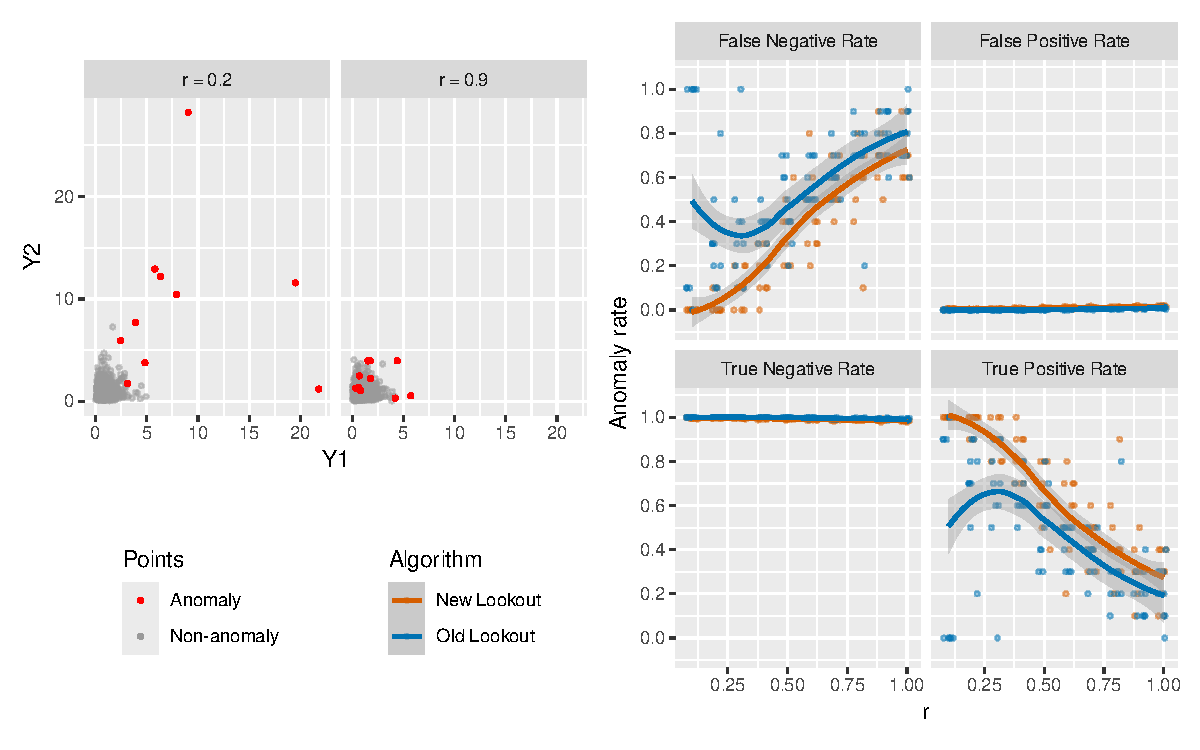
\includegraphics[width=\textwidth]{Figures/Exp1_Gamma_Rates.pdf}
  \caption{Experiment 1. Left: data with $r = 0.2$ and $r = 0.9$; anomalies with lower values of $r$ are easier to identify. Right: error rates of the two versions of lookout, with points jittered horizontally.}
  \label{fig:exp1}
\end{figure}

\cref{fig:exp1} shows the data and results. As $r$ increases the anomalies become more similar to the non-anomalies, so the true positive rate falls. The new version has a higher true positive rate than the original at every value of $r$ below 1, with the largest difference at $r=0.1$ (0.97 against 0.19), where the anomalies are farthest from the non-anomalous observations. Both versions have false positive rates of at most 0.012.

\subsection[Experiment 2: Anomalies on the boundary as n increases]{Experiment 2: Anomalies on the boundary as $n$ increases}

The non-anomalous observations have independent $\mathcal{N}(0,1)$ coordinates in $\R^2$, with $n \in \{1000, 2000, \ldots, 10000\}$, and there are $0.005n$ anomalies in a ring just beyond most of them. The anomaly means $\bm{\mu}_i$ lie on the circle of radius $2.2\sqrt2$ about the origin, with $\mu_{i1} \sim \mathcal{U}(-2.2\sqrt2, 2.2\sqrt2)$ and $\mu_{i2}$ negative for a randomly chosen half of the anomalies, and $Y_{ij} \sim \mathcal{N}(\mu_{ij}, 0.1^2)$ for $j=1,2$. There are 10 replications for each $n$, and for both versions the kernel density estimates use the truncated sum described in \cref{sec:modified}, with 100 neighbours.

\begin{figure}[!b]
  \centering
  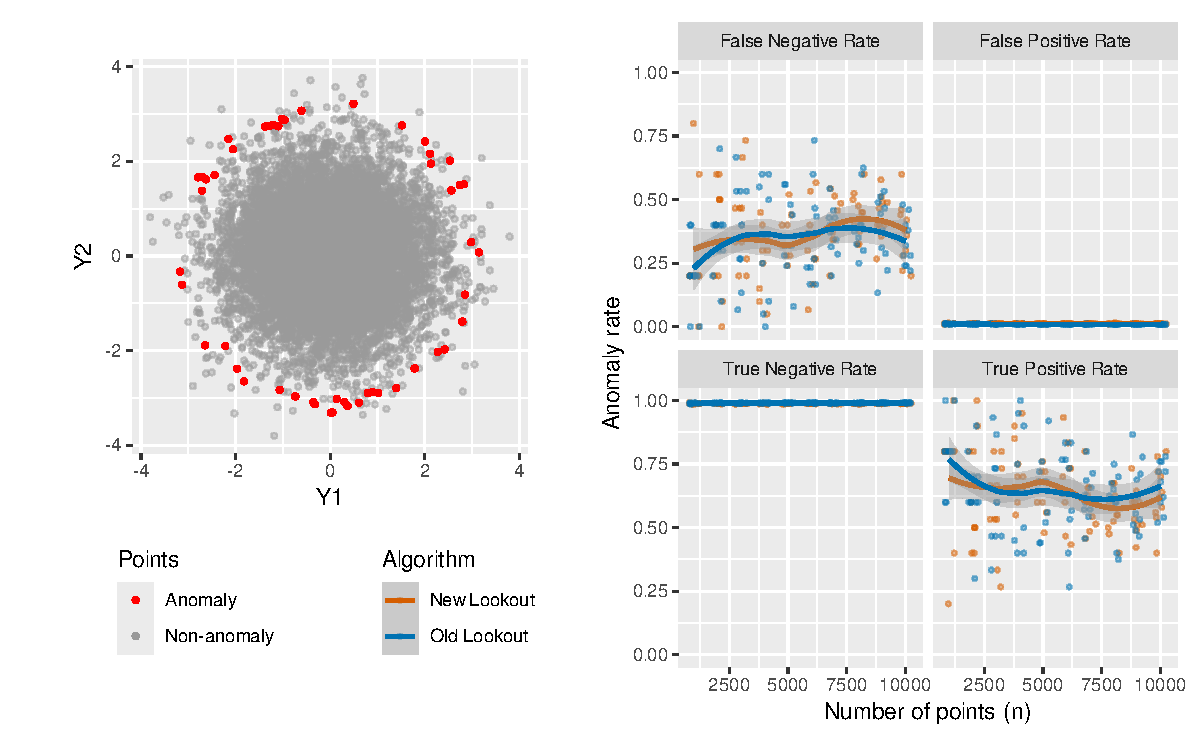
\includegraphics[width=\textwidth]{Figures/Exp2.pdf}
  \caption{Experiment 2. Left: data for $n=10000$. Right: error rates of the two versions of lookout, with points jittered horizontally.}
  \label{fig:exp2}
\end{figure}

\cref{fig:exp2} shows the data of one replication and the results. The false positive rates are about 0.012 for the new version and 0.010 for the original. The two versions have similar true positive rates at every $n$, between about 0.55 and 0.8. The online Appendix repeats this experiment with gamma-distributed observations (Experiment S2); there the two versions differ little, and the original is slightly better at the largest sample sizes.

\subsection{Experiment 3: Normal distributions moving out in each iteration}

The sample has 405 points in $\R^6$, of which five are anomalies. The non-anomalies are $\mathcal{N}(0,1)$ in every dimension. The anomalies differ from the non-anomalies only in the first dimension, where they are $\mathcal{N}(1.5 + 0.5i,\, 0.2^2)$ at iteration $i \in \{1, \ldots, 10\}$, so they move further from the non-anomalous points at each iteration. Each iteration is repeated 10 times.

\begin{figure}[!b]
  \centering
  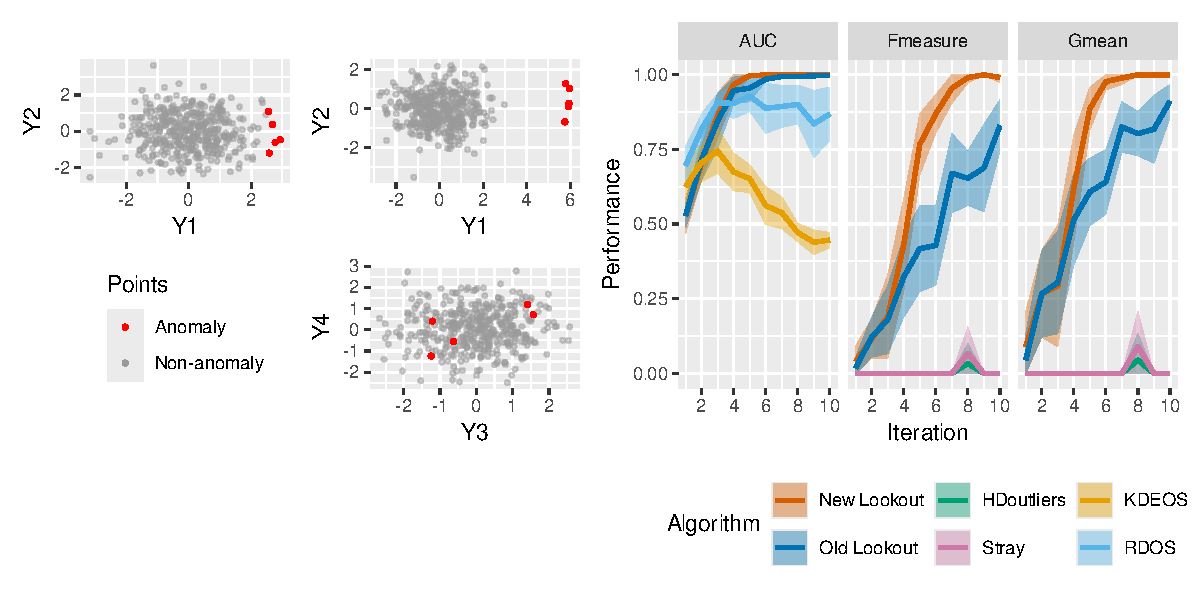
\includegraphics[width=\linewidth]{Figures/Exp3_Data_and_Results.pdf}
  \caption{Experiment 3. Left: the $Y_1Y_2$ plane at the third iteration, with anomalies in red. Middle: the $Y_1Y_2$ (top) and $Y_3Y_4$ (bottom) planes at the ninth iteration. Right: mean AUC, Fmeasure and Gmean over ten replications, with bands of $\pm2$ standard errors, for the two versions of lookout, HDoutliers, KDEOS, RDOS and stray.}
  \label{fig:exp3}
\end{figure}

\cref{fig:exp3} shows the data at the third and ninth iterations, and the results. By the ninth iteration the anomalies have separated from the other points in the $Y_1$ direction, but they remain mixed with them on the $Y_3Y_4$ plane. The new version has higher Fmeasure and Gmean than the original from the fourth iteration, and the two versions have similar AUC. RDOS has the highest AUC in the first three iterations; from the fourth, both versions of lookout are at least as good as the four other methods on every metric.

\subsection[Experiment 4: Annulus in R3]{Experiment 4: Annulus in $\R^3$}

\begin{figure}[!b]
  \centering
  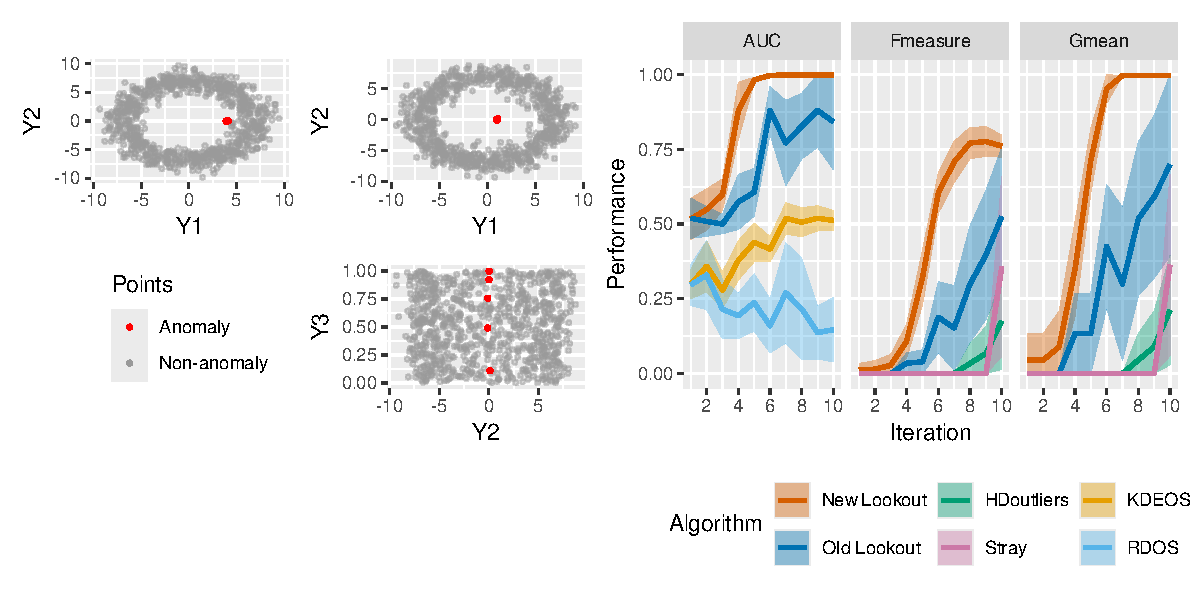
\includegraphics[width=\linewidth]{Figures/Exp4_Data_and_Results.pdf}
  \caption{Experiment 4. Left: the $Y_1Y_2$ plane at the third iteration, with anomalies in red. Middle: the $Y_1Y_2$ (top) and $Y_2Y_3$ (bottom) planes at the ninth iteration. Right: mean AUC, Fmeasure and Gmean over ten replications, with bands of $\pm2$ standard errors, for the two versions of lookout, HDoutliers, KDEOS, RDOS and stray.}
  \label{fig:exp4}
\end{figure}

The sample has 805 points in $\R^3$, of which five are anomalies. On the $Y_1Y_2$ plane the non-anomalies lie in an annulus, with uniform angle and $\mathcal{N}(7, 1)$ radius, and $Y_3 \sim \mathcal{U}(0,1)$ for all points. At iteration $i \in \{1, \ldots, 10\}$ the anomalies have $Y_1 \sim \mathcal{N}(5.5 - 0.5i,\, 0.1^2)$ and $Y_2 \sim \mathcal{N}(0, 0.1^2)$, so they move from the inner edge of the annulus towards the centre of the hole. Each iteration is repeated 10 times. \cref{fig:exp4} shows the data at iterations 3 and 9 and the results. The AUC and Gmean of the new version are close to one from the seventh iteration, when it identifies all five anomalies in every replication; its Fmeasure levels off at about 0.77 because of false positives. The original version is lower and more variable, KDEOS and RDOS have AUC of at most about 0.5 throughout, and HDoutliers and stray identify almost no anomalies before the eighth and tenth iterations respectively.

\subsection[Experiment 5: Unit cube in R20]{Experiment 5: Unit cube in $\R^{20}$}

The sample has 500 points in $\R^{20}$, of which one is an anomaly. Initially all 500 points are uniform on $(0,1)$ in each dimension. At iteration $i \in \{1, \dots, 20\}$ the first $i$ coordinates of the anomaly are set to $0.9$, so that at iteration 20 it is $(0.9, \dots, 0.9)$, and each iteration is repeated 10 times. The anomaly is not anomalous in any single coordinate, on any $Y_iY_j$ plane or in the first two principal components, so \cref{fig:exp5} shows the $D_1D_2$ plane of the projection given by \textit{dobin} \citep{dobinPaper}, a dimension reduction method designed for anomalies, at iterations 5, 12 and 20, together with the results. The anomaly is mixed with the other points at iteration 5 and separated from them at iterations 12 and 20. Both versions of lookout are run without scaling. The AUC of the new version is close to one from the twelfth iteration except at the fourteenth, and that of RDOS from about the eleventh; the original version and KDEOS are lower. The Gmean of the new version is close to one from the sixteenth iteration, when it identifies the anomaly in every replication. Its Fmeasure stays below 0.5 because of about three false positives among the 499 non-anomalies. HDoutliers and stray never identify the anomaly.

\begin{figure}[!tb]
  \centering
  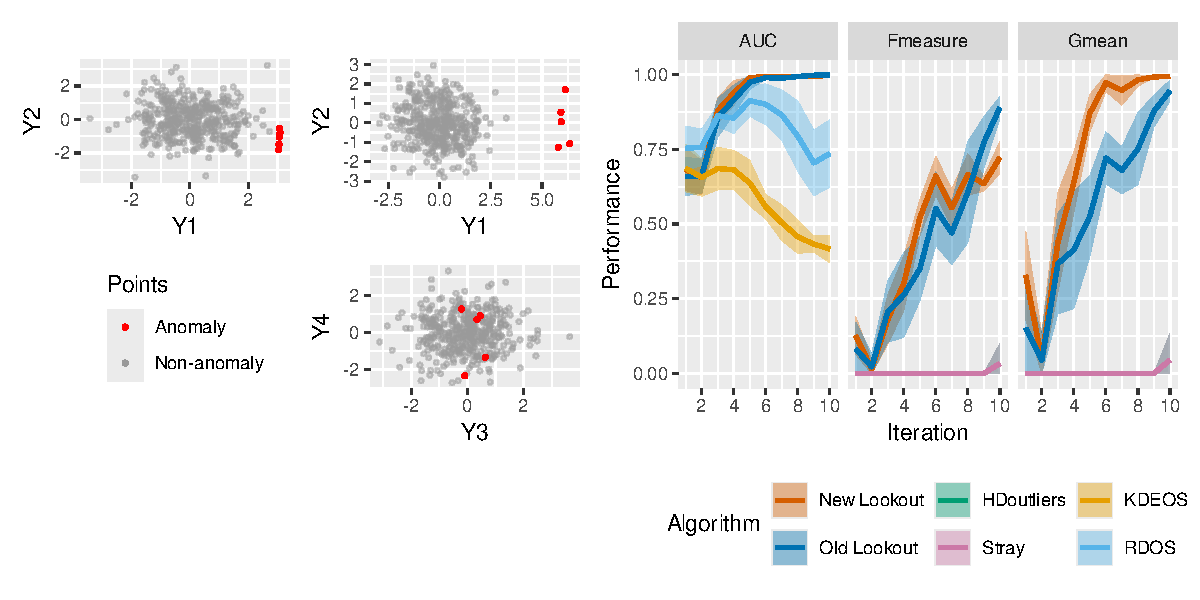
\includegraphics[width=\linewidth]{Figures/Exp5_Data_and_Results.pdf}
  \caption{Experiment 5. Left: the $D_1D_2$ plane of the dobin projection at the fifth, twelfth and twentieth iterations, with the anomaly in red. Right: mean AUC, Fmeasure and Gmean over ten replications, with bands of $\pm2$ standard errors, for the two versions of lookout, HDoutliers, KDEOS, RDOS and stray.}
  \label{fig:exp5}
\end{figure}

\subsection{Sensitivity to the bandwidth}\label{sec:bwablation}

\cref{sec:whynotmise} argues that the bandwidth should be of the order of the spacing in the tails, and that neither the constant nor MISE-optimality matters much. To check this, we repeated Experiments 1, 2 and 3, and Experiment S1 of the online Appendix, with $h_n$ multiplied by $1/4$, $1/2$, $2$ and $4$, and with $h_n$ replaced by the AMISE-optimal bandwidth $h_{\text{opt}}$ of \cref{tab:bwconst}. The details and results are in the online Appendix. The area under the ROC curve was almost the same for every bandwidth from $h_n/2$ to $4h_n$, so the ranking of the observations is insensitive to the bandwidth. The threshold is more sensitive. At $h_n$ the false positive rate was close to the nominal $\alpha=0.01$, and at $h_n/4$ it was between $0.05$ and $0.27$, because observations with no other observation inside the kernel support are all declared anomalous. With $h_{\text{opt}}$ the results were similar to those at $h_n$ for normal data in two dimensions. In six dimensions $h_{\text{opt}}$ was about a quarter of $h_n$.

% -------------------------------------------------------------------------
\section{Applications}\label{sec:applications}
% -------------------------------------------------------------------------

We apply the new and original versions of lookout to two real datasets. Neither has labelled anomalies, so accuracy cannot be measured, but both have two variables, so the output can be inspected.
\begin{enumerate}
  \item Old Faithful dataset\footnote{Data downloaded from \url{https://geysertimes.org}.}: 2,097 eruptions of the Old Faithful Geyser in Yellowstone National Park, Wyoming, USA, from 14 January 2017 to 29 December 2023. For each recorded eruption the duration is given in seconds along with the waiting time to the following eruption. The records are incomplete, especially during winter.
  \item Wine reviews dataset\footnote{Data downloaded from \url{https://www.kaggle.com/datasets/zynicide/wine-reviews/data}.}: 110,203 reviews of wines from 42 countries, obtained from the \emph{Wine Enthusiast Magazine} during the week of 15 June 2017. We use the 4,496 wines labelled Shiraz or Syrah, and two variables: the points score given by the \emph{Wine Enthusiast} reviewer on a scale of 0--100, and the price of a bottle. The kernel density estimates use the truncated sum described in \cref{sec:modified}, with 100 neighbours.
\end{enumerate}

\begin{figure}[!htb]
  \centering
  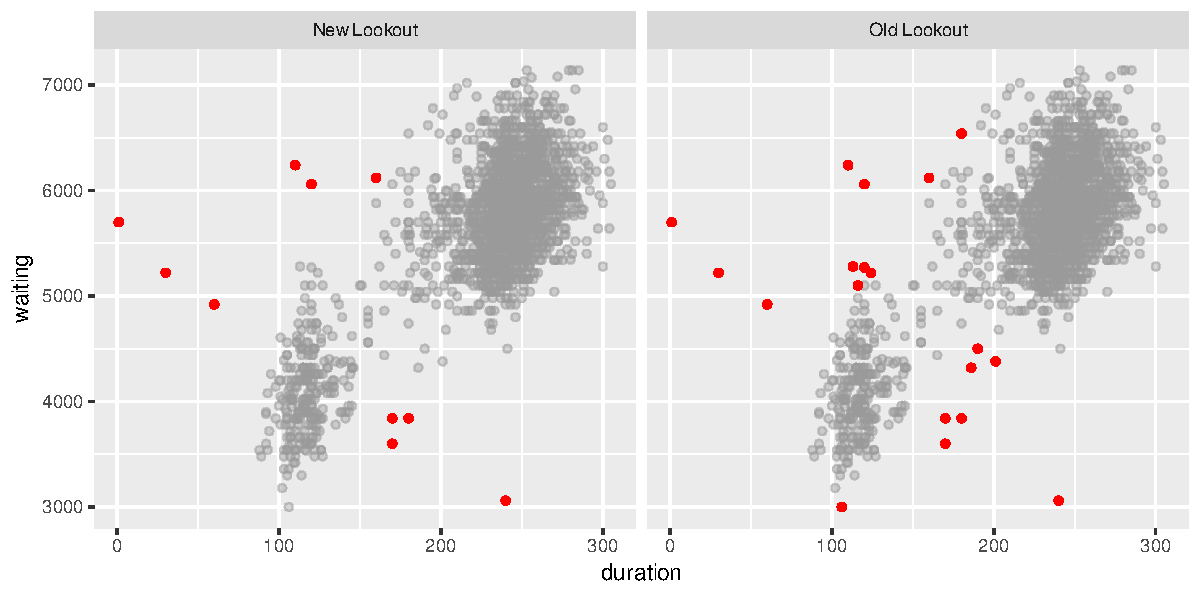
\includegraphics[width=0.8\linewidth]{Figures/old_faithful.pdf}
  \caption{Anomalies (red) identified in the Old Faithful data by the new version of lookout (left) and the original version (right).}
  \label{fig:oldfaithful}
\end{figure}

\begin{figure}[!htb]
  \centering
  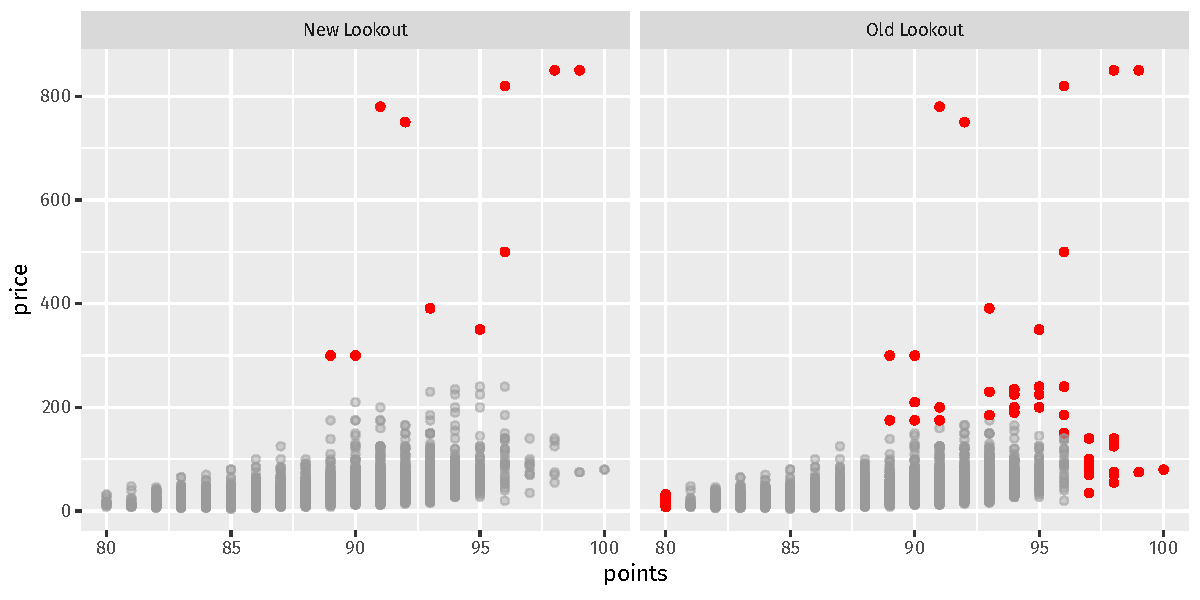
\includegraphics[width=0.8\linewidth]{Figures/wine_reviews.pdf}
  \caption{Anomalies (red) identified in the wine reviews data by the new version of lookout (left) and the original version (right).}
  \label{fig:winereviews}
\end{figure}

\cref{fig:oldfaithful} shows the Old Faithful data. The new version identifies the observations in the sparse regions between and around the two clusters. The original identifies fewer of those, and instead flags a group of observations at the lower edge of the smaller cluster, close to the bulk of the data.

\cref{fig:winereviews} shows the wine reviews. The new version identifies the expensive wines and little else. The original also flags many wines with the highest and lowest scores at ordinary prices, and several at the edge of the main cloud. In both datasets the new version flags the observations that are isolated in the two-dimensional space, and the original flags observations at the margins of the dense regions as well; we regard the former as the more useful behaviour.

% ---------------------------------------------------------------------------
\section{Discussion and conclusions (SK)}\label{sec:conclusion}
% ---------------------------------------------------------------------------


\section*{Supplementary material}

The online Appendix contains the proofs of \cref{prop:order} and \cref{cex:fattails}, two further comparisons of the original and modified algorithms, and a set of showcase examples. The updated algorithm is implemented in the \texttt{lookout} R package \citep{Rlookout}, available on CRAN at \url{https://CRAN.R-project.org/package=lookout}. Files to reproduce all numerical examples are available at \url{https://github.com/robjhyndman/lookout2}.

%% Add an Acknowledgements section here if there is anyone to thank.

\section*{Funding}

Rob Hyndman and Sevvandi Kandanaarachchi are part of the Australian Research Council Industrial Transformation Training Centre in Optimisation Technologies, Integrated Methodologies, and Applications (OPTIMA), Project ID IC200100009. Katharine Turner is supported by an Australian Research Council Future Fellowship, FT250100951.

\section*{Disclosure statement}

The authors report there are no competing interests to declare.

\bibliography{References}

\end{document}
